\documentclass[usenames,dvipsnames,french]{beamer}

\mode<presentation> {

\usetheme{Montpellier}
}

\usepackage{graphicx} % Allows including images
\usepackage[frenchb]{babel}
\usepackage[T1]{fontenc}
\usepackage[utf8]{inputenc}
% \usepackage[demo]{graphicx}
% \usepackage{caption}

\usepackage{subcaption}
% \usepackage{subfig}
% \usepackage{algorithm,algorithmic}
\usepackage{algorithm2e}
\usepackage{listings}
% \usepackage{ntheorem}
\usepackage{booktabs} % Allows the use of \toprule, \midrule and \bottomrule in tables
\setcounter{tocdepth}{2}
\graphicspath{{../../Figures/}}


\DeclareMathOperator*{\argmin}{arg\,min}
\DeclareMathOperator*{\argmax}{arg\,max}
\newtheorem*{proposition}{Proposition}

% exercices comptés
\newcounter{numexos}%Création d'un compteur qui s'appelle numexos
\setcounter{numexos}{0}%initialisation du compteur
\newcommand{\exercice}[1]{%Création d'une macro ayant un paramètre
\addtocounter{numexos}{1}%chaque fois que cette macro est appelée, elle ajoute 1 au compteur numexos
\textcolor{DarkOrchid}{Exercice\,\thenumexos\,:}\,#1%Met en rouge Exercice et la valeur du compteur appelée par \thenumeexos
}
%----------------------------------------------------------------------------------------
%	TITLE PAGE
%----------------------------------------------------------------------------------------

\setbeamertemplate{title page}{
    \centering

    \Large\bfseries
    Machine learning Tek 5: classification, logistic regression
    

\begin{figure}[!h]

\includegraphics[width=8cm]{separation}
\end{figure}

    }
\begin{document}

\frame{\titlepage}

\begin{frame}{Content}

    \tableofcontents

\end{frame}

\section{The binary classification problem}%
\label{sec:classification}

\subsection{Problem statement}%
\label{sub:problem_statement}

\begin{frame}{General classification problem}

    \textbf{Classification:} supervised learning in which we predict a \textbf{class} (the set of possible labels is discrete (most often \textbf{finite})).

    \begin{itemize}
        \item $ \mathcal{X} = \mathbb{R}^d$
	\item $ \mathcal{Y}  = \{-1, 1\}$ or $ \mathcal{Y}  = \{0, 1\}$ for \textbf{binary} classification ($2$ possible classes).
	\item $l(y,z) = 1_{y\neq z}$ ("0-1" loss)

	    \url{https://en.wikipedia.org/wiki/Indicator_function} 

	\item $F = \mathcal{Y}^{ \mathcal{X} }$
	\item Examples: MNIST, ImageNet
    \end{itemize}
\end{frame}

\begin{frame}{Empirical risk}

    We learn from a dataset $D_n$ of $n$ \textbf{labeled examples}; 
\begin{equation}
    D_n =\{(x_i,y_i), i\in[1, n]\}
\end{equation}

If the dataset is split into a train and a test set, and with the "0-1" loss, the train error writes

	    \begin{equation}
		\frac{1}{n_{\text{train}}}\sum_{(x_i, y_i)\in (X_{train}\times y_{train})} 1_{{\tilde{f}(x_i)\neq y_i}}
	    \end{equation}

	    \exercice{}What is a natural interpretation of the train error with the "0-1" loss ?
	    \\

	    The \textbf{accuracy} is $1-\text{train error}$.
\end{frame}


\begin{frame}
    Let us compare the classification train error to the squared-loss train error that we studied last week:

    \begin{itemize}
    	\item classification with "0-1" loss:
	    \begin{equation}
		\frac{1}{n_{\text{train}}}\sum_{(x_i, y_i)\in (X_{train}\times y_{train})} 1_{{\tilde{f}(x_i)\neq y_i}}
	    \end{equation}
	\item regression with squared-loss:
	    \begin{equation}
		\frac{1}{n_{\text{train}}}\sum_{(x_i, y_i)\in (X_{train}\times y_{train})} (\tilde{f}(x_i)-y_i)^2
	    \end{equation}
    \end{itemize}

    We have not yet focused much on the optimization side of ML. But to find a good $\tilde{f}$, we have discussed \textbf{empirical risk minimization}, which consists in finding $\tilde{f}$ such that the train error is as small as possible, while avoiding overfitting at the same time.

    As we will see next week, the possibility to differentiate the train error with respect to $ \tilde{f}$ is one of the building blocks of the optimization process.

\end{frame}

\begin{frame}
    Let us compare the classification train error to the squared-loss train error that we studied last week:

    \begin{itemize}
    	\item classification with "0-1" loss:
	    \begin{equation}
		\frac{1}{n_{\text{train}}}\sum_{(x_i, y_i)\in (X_{train}\times y_{train})} 1_{{\tilde{f}(x_i)\neq y_i}}
	    \end{equation}
	\item regression with squared-loss:
	    \begin{equation}
		\frac{1}{n_{\text{train}}}\sum_{(x_i, y_i)\in (X_{train}\times y_{train})} (\tilde{f}(x_i)-y_i)^2
	    \end{equation}
    \end{itemize}

    The issue is that differentiating the train error with respect to the "0-1" loss is \textbf{not informative} ! The derivative is $0$ almost everywhere.


\end{frame}


% \begin{frame}{Bayes predictor}
% 
%     \begin{proposition}{Law of total expectation}
% 
% 	\begin{equation}
% 	    E_{X,Y}\Big[l(X,Y)\Big] = E_X\Big[ E\big(l(X,Y)|X \big) \Big]
% 	\end{equation}
%     \end{proposition}
% 
%     $E\big(l(X,Y)|X \big) $ is the expectation of $l(X, Y)$ given $X$.
% 
%     
% \end{frame}
% 
% \begin{frame}{Bayes predictor}
% Hence, 
%     
% \begin{equation}
%     f^*(x)= \argmin_{z\in \mathcal{Y} }E\Big[l(y,z)|X=x\Big]
% \end{equation}
% \end{frame}
% 
% \begin{frame}{Bayes predictor}
%     \textbf{{Reminder}} : if we assume the knowledge of the joint distribution $(X,Y)$, the Bayes predictor can be explicitely computed. 
% 
%     \begin{equation}
%         \begin{aligned}
%             \label{eq:}
% 	    f^*(x)&= \argmin_{z\in \mathcal{Y} }E_Y\Big[l(Y,z)|X=x\Big]\\
% 	    &= \argmin_{z\in \mathcal{Y} }P(Y\neq z|X=x)\\
% 	    &= \argmin_{z\in \mathcal{Y} }1-P(Y=z|X=x)\\
% 	    &= \argmax_{z\in \mathcal{Y} }P(Y=z|X=x)
%         \end{aligned}
%     \end{equation}
% 
%     The optimal classifier selects the most probable output given $X=x$.
% \end{frame}
% 
% \begin{frame}{Bayes risk}
%     \begin{equation}
%         \begin{aligned}
%             \label{eq:}
%             R^* &= E_{(X,Y)}\Big[ l(Y, f^*(X)) \Big]\\
% 	    &= E_X\Big[E\Big(l(Y\neq f^*(X)|X\Big) \Big]\\
% 	    &= E_X\Big[P(Y\neq f^*(X)|X) \Big]\\
%         \end{aligned}
%     \end{equation}
% \end{frame}
% 
% \begin{frame}{Bayes risk}
%     \begin{equation}
%         \begin{aligned}
%             \label{eq:}
% 	    R^* &= E\Big[ l(Y, f^*(X)) \Big]\\
% 	    &= E_X\Big[E_Y\Big(l(Y\neq f^*(X)|X\Big) \Big]\\
% 	    &= E_X\Big[P(Y\neq f^*(X)|X) \Big]\\
%         \end{aligned}
%     \end{equation}
% 
%     But we have
% 
%     \begin{equation}
%         \begin{aligned}
%             \label{eq:}
% 	    P\big(Y\neq f^*(X)|X=x\big)&= P\big( Y\neq f^*(x)\big)
% 	    %E_X\Big[ P(Y\neq f^*(x)|X=x) \Big] &= E_X\Big[\min(\eta(x), 1-\eta(x)\Big]\\
%         \end{aligned}
%     \end{equation}
% \end{frame}
% 
% \begin{frame}{Bayes risk}
%     We note $\eta(x) = P(Y=1|X=x)$. Then, 
%     \begin{itemize}
%         \item If $ \eta(x)> \frac{1}{2} $, then $f^*(x)=1$, and $P\big( Y\neq f^*(x)\big) =   P\big( Y=0\big)=1-\eta(x)$
% 	\item If $ \eta(x)< \frac{1}{2} $, then $f^*(x)=0$, and $P\big( Y\neq f^*(x)\big) =   P\big( Y=1\big)=\eta(x)$
%     \end{itemize}
% 
%     In both cases, $P\big( Y\neq f^*(x)\big)= \min(\eta(x), 1-\eta(x))$.
% 
%     We conclude that 
% 
%     \begin{equation}
% 	R^* = E_X\Big[ \min(\eta(X), 1-\eta(X))\Big]
%     \end{equation}
% \end{frame}
% 
% \begin{frame}{}
%     \exercice{} Same random variable $(X,Y)$ as in lecture $3$, with $p=1/3$, $q=3/4$.
%     \begin{itemize}
% 	\item $ \mathcal{X} = \{0, 1\}$, $ \mathcal{Y}  = \{0, 1\}$.
%         \item 
%             $ X\sim B( \frac{1}{2} )$, 
%          $$
%             Y = \left\{
%                 \begin{array}{ll}
%                     B(1/3) \text{ if } X=1   \\
%                     B(3/4) \text{ if } X=0   \\
%                 \end{array}
%                 \right.
%                 $$
%     With $B(p)$ a Bernoulli law with parameter $p$.
%     \end{itemize}
%     Compute the Bayes estimator and the bayes risk.
% \end{frame}
% 
% \begin{frame}{Bayes estimator}
%     Bayes estimator
% \begin{itemize}
%     \item $f^*(0)=1$
%     \item $f^*(1)=0$
% \end{itemize}
% 
% \begin{itemize}
%     \item $\eta(1) = \frac{1}{3} $
%     \item $\eta(0) = \frac{3}{4} $
% \end{itemize}
% 
% \begin{equation}
%     R^* = \frac{7}{24} 
% \end{equation}
% 
% \end{frame}
% 
\begin{frame}{Real-valued function}

    Instead of an application that predicts $-1$ or $1$, we will learn $g: \mathcal{X} \rightarrow \mathbb{R} $ and define $ f(x) = \text{sign}(g(x))$ with
    
         $$
	    \text{sign}(x) = \left\{
                \begin{array}{ll}
                    1 \text{ if } x\geq 0   \\
		    -1 \text{ if } x<0   \\
                \end{array}
                \right.
                $$
\end{frame}

% \begin{frame}{Risk}
%
%     The risk (generalization error) of $f = \text{sign} \circ g$ writes:
%
%     \begin{equation}
%         \begin{aligned}
%             \label{eq:}
% 	    R(g) &= P( \text{sign}(g(x))\neq y)\\
% 	    &= E\Big[1_{\text{sign}(g(x))\neq y} \Big]\\
% 	    &= E\Big[ 1_{yg(x)<0} \Big]
%         \end{aligned}
%     \end{equation}
% \end{frame}

% \begin{frame}{Several solutions}
%
%     There might be many optimal maps $g$, i.e: such that $ \text{sign}(g(x)) = f^*(x)$ for all $x$.
%     \\
%
%     (Here, $f^*(x)$ is the Bayes predictor, which is the optimal predictor: it minimizes the generalization error (risque réel))
%
%     
% \end{frame}

% \begin{frame}{Margin based 0-1 loss function $ \Phi_{0-1}$}
%     \begin{equation}
%         \begin{aligned}
%             \label{eq:}
% 	    R(g) &= E\Big[1_{\text{sign}(g(x))\neq y} \Big]\\
% 	    &= E\Big[ 1_{yg(x)<0} \Big]\\
% 	    &= E\Big[ \Phi_{0-1}(yg(x)) \Big]
%         \end{aligned}
%     \end{equation}
%
%     \begin{figure}[htpb]
%         \centering
%         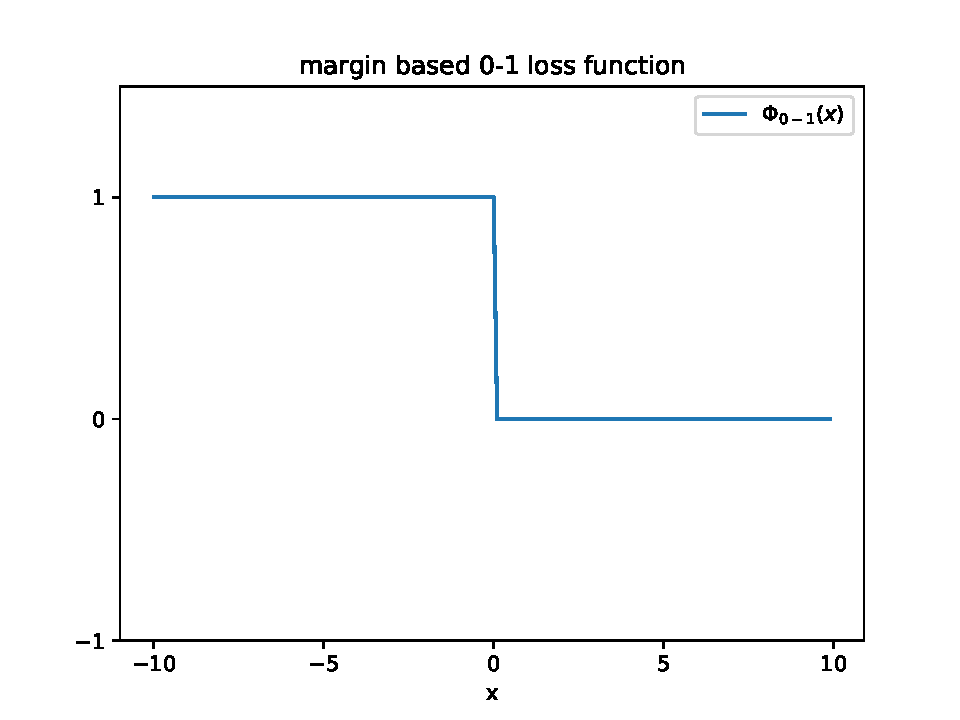
\includegraphics[width=0.5\linewidth]{margin}
%         \label{fig:margin}
%     \end{figure}
%     
% \end{frame}

\begin{frame}{Empirical risk minimization}

    The corresponding empirical risk writes ($\Phi_{0-1}$ is defined by the image):

\begin{equation}
    \frac{1}{n} \sum^{n}_{i=1} \Phi_{0-1}(y_ig(x_i))
\end{equation}
    
    \begin{figure}[htpb]
        \centering
        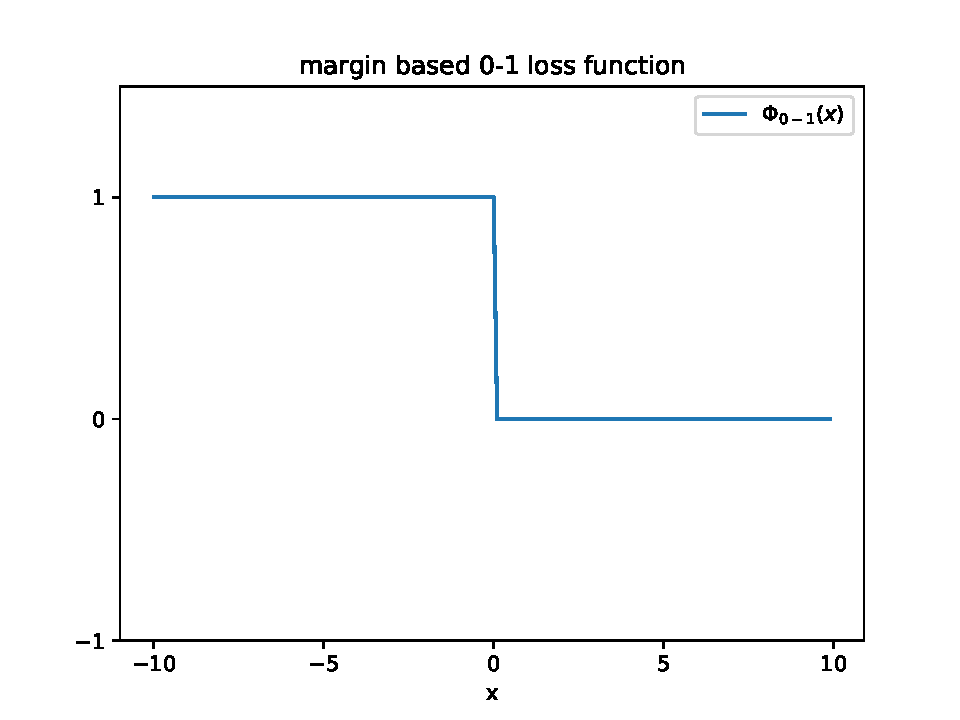
\includegraphics[width=0.5\linewidth]{margin}
        \label{fig:margin}
    \end{figure}

\end{frame}


\subsection{Convexification of the risk and calibration}%
\label{sub:convexification_of_the_risk}

\begin{frame}{Convex surrogate}
    Key idea: replace $ \Phi_{0-1}$ by another function $\Phi$ that is easier to optimize (convex, differentiable) but still represents the correctness of the classification.

    Natural question: but does minimizing the $\Phi$-risk lead to a good "0-1" loss prediction ? Often yes, but answering this question in detail requires an advanced study.

    \begin{figure}[htpb]
        \centering
        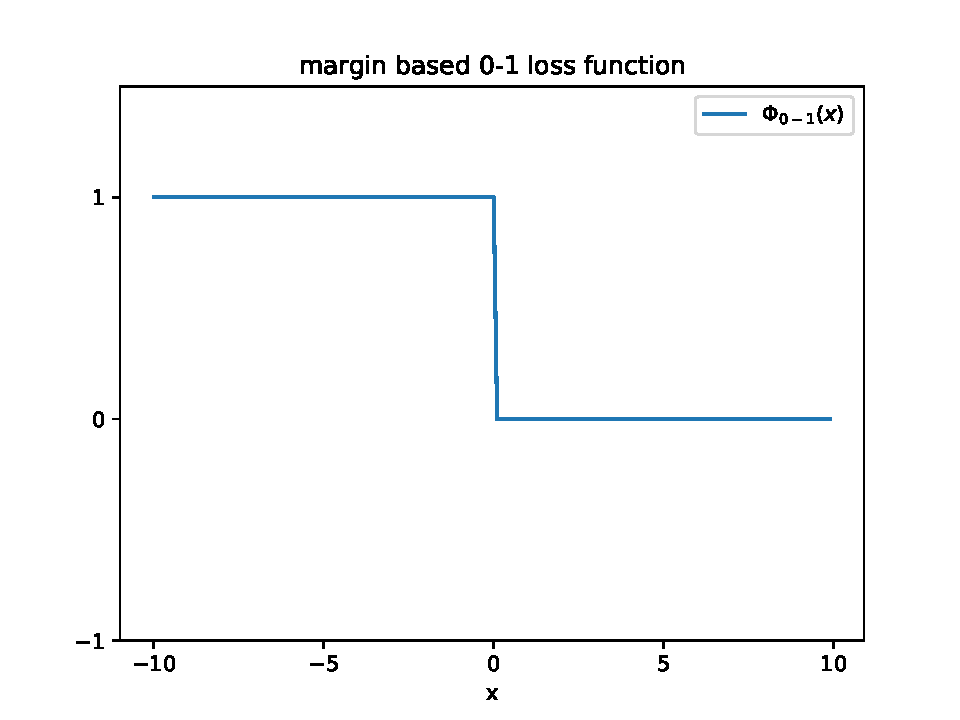
\includegraphics[width=0.3\linewidth]{margin}
        \label{fig:margin}
    \end{figure}
\end{frame}

\begin{frame}{Most common convex surrogates}

    \begin{definition}{Logistic loss}
    \label{loss:logistic}
	\begin{equation}
	    \Phi(u) = \log(1+e^{-u})
	\end{equation}
    \end{definition}

    With linear predictors ($g(x_i)= \langle \theta, x_i \rangle$), this loss will lead to \textbf{{logistic regression}} (which is classification despite its name).
    
\end{frame}

\begin{frame}{Most common convex surrogates}

    If $ \mathcal{Y}= \{0, 1\}$, $ \hat{y}$ is the prediction and $y$ is the correct label, then we sometimes write:

	\begin{equation}
	    l(\hat{y}, y) = y\log(1+e^{- \hat{y}})+ (1-y)\log(1+e^{ \hat{y}})
	\end{equation}
    (cross entropy loss)
    
\end{frame}

\begin{frame}{Logistic function}
    \begin{figure}[htpb]
        \centering
        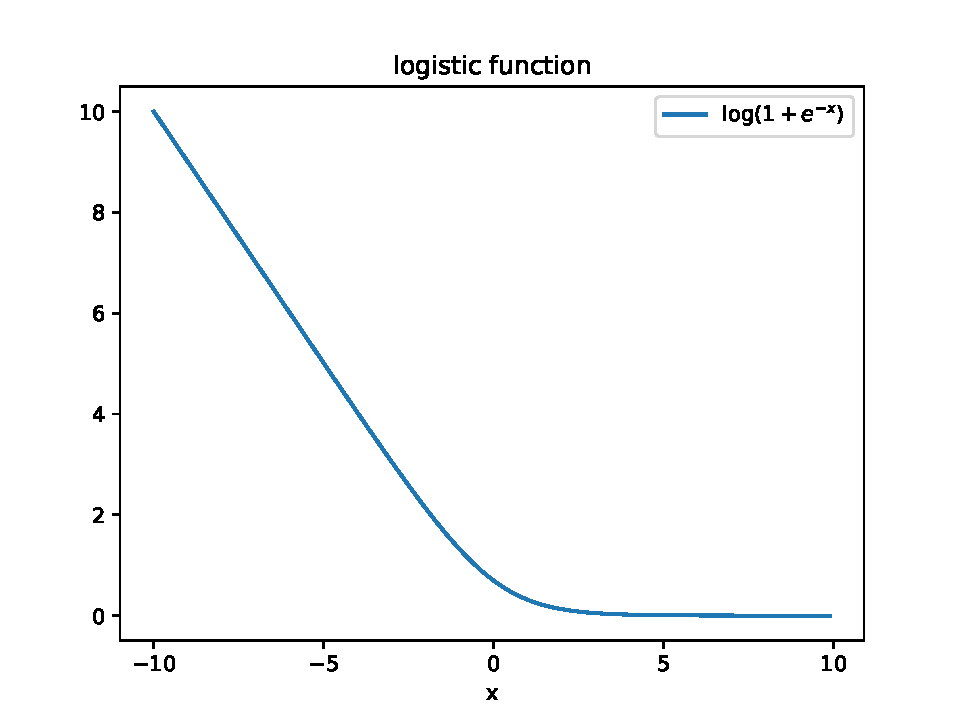
\includegraphics[width=0.8\linewidth]{logistic}
        \label{fig:logistic}
    \end{figure}
\end{frame}

% \begin{frame}{Most common convex surrogates}
%
%     \begin{definition}{Hinge loss}
% 	\begin{equation}
% 	    \Phi(u) = max(1-u, 0) 
% 	\end{equation}
%     \end{definition}
%
%     With linear predictors, this loss will lead to \textbf{{Support vector machines}}.
%
%     \begin{definition}{Squared hinge loss}
% 	\begin{equation}
% 	    \Phi(u) = (max(1-u, 0))^2
% 	\end{equation}
%     \end{definition}
%     
% \end{frame}

\begin{frame}{Hinge loss}
    \begin{figure}[htpb]
        \centering
        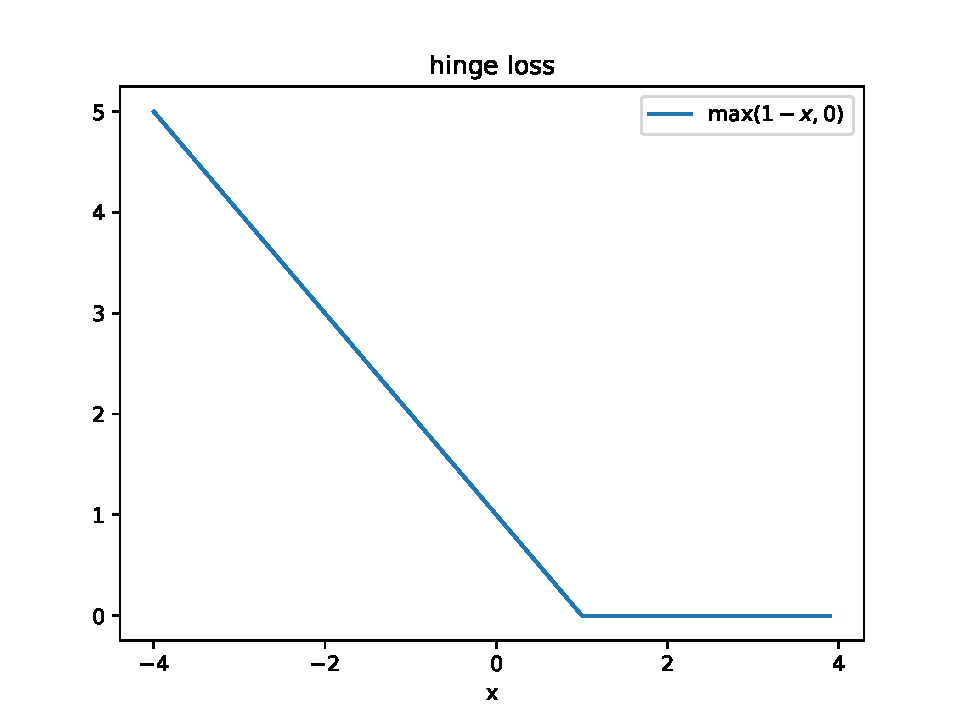
\includegraphics[width=0.8\linewidth]{hinge}
        \label{fig:hinge}
    \end{figure}
\end{frame}

%\begin{frame}{$\Phi$-risk minimization}
%
%    \begin{itemize}
%        \item We come back to the question: does minimizing the empirical $\Phi$-risk lead to a good "0-1" loss prediction ?
%	\item The Bayes predictor stays the same, but several $\Phi$ can be used. Hence, several minimizers can be obtained, since the minimizer or the $\Phi$-risk depends on the choice of $\Phi$.
%    \end{itemize}
%    
%\end{frame}
%
%\begin{frame}{$Phi$-risk minimization}
%
%    \begin{itemize}
%        \item Testing error
%	    \begin{equation}
%		R(g) = E\Big[ \Phi_{0-1}(yg(x)) \Big]
%	    \end{equation}
%	\item Testing loss
%	    \begin{equation}
%		R_{\Phi}(g) = E\Big[ \Phi(yg(x))\Big]
%	    \end{equation}
%    \end{itemize}
%\end{frame}
%
%\begin{frame}{Conditional $\Phi$-risk}
%
%    \begin{definition}{Conditional $\Phi$-risk}
%	\begin{equation}
%	    E\Big[\Phi(yg(x))|x \Big]=\eta(x)\Phi(g(x))+(1-\eta(x))\Phi(-g(x)) = C_{\eta(x)}(g(x))
%	\end{equation}
%	with
%	\begin{equation}
%	    C_{\eta}(\alpha) = \eta \Phi(\alpha) + (1-\eta)\Phi(-\alpha)
%	\end{equation}
%    \end{definition}
%    
%\end{frame}
%
%\begin{frame}{Calibrated $\Phi$}
%    We say that $\Phi$ is \textit{{calibrated}} if:
%    \begin{itemize}
%	\item $\eta > \frac{1}{2} \Leftrightarrow \argmin_{\alpha\in \mathbb{R} }C_{\eta}(\alpha)\subset \mathbb{R}^*_+$
%	\item $\eta < \frac{1}{2} \Leftrightarrow \argmin_{\alpha\in \mathbb{R} }C_{\eta}(\alpha)\subset \mathbb{R}^*_-$
%    \end{itemize}
%    This means that the optimal $\forall x$, taken independently, the optimal $g(x)$ obtained by minimizing the conditional $\Phi$-risk leads to the same prediction as the Bayes predictor.
%    
%\end{frame}
%
%\begin{frame}{Necessary and sufficient condition}
%
%    \begin{proposition}
%        Let $\Phi: \mathbb{R} \rightarrow \mathbb{R} $ convex.
%
%	$\Phi$ is calibrated $ \Leftrightarrow \Phi$ is differentiable at $0$ and $\Phi'(0)<0$.
%    \end{proposition}
%    
%\end{frame}
%
%\begin{frame}{Necessary and sufficient condition}
%
%    \begin{proposition}
%        Let $\Phi: \mathbb{R} \rightarrow \mathbb{R} $ convex.
%
%	$\Phi$ is calibrated $ \Leftrightarrow \Phi$ is differentiable at $0$ and $\Phi'(0)<0$.
%    \end{proposition}
%    
%    The conditions are verified for the logistic loss and the hinge loss.
%\end{frame}
%
%\begin{frame}{Calibration function}
%
%    To know if minimizing $R_{\Phi}(g)$ leads to minimizing $R(g)$, it would be sufficient to have a monotonic function $H$ (calibration function), such that
%    \begin{equation}
%	R(g)-R^*\leq H\Big[R_{\Phi}(g)-R_{\Phi}^* \Big] 
%    \end{equation}
%    
%\end{frame}
%
%
%
\subsection{Logistic regression}%
\label{sub:logistic_regression}

\begin{frame}{Logistic regression}
    
    \begin{itemize}
        \item $ g(x) = \langle x, \theta \rangle = x^T \theta $.
	\item $f(x) = \text{sign}( \langle  x^T\theta \rangle )$
	\item It can be seen as "linear regression applied to classification".
    \end{itemize}
\end{frame}

\section{Applications}

\subsection{Toy dataset}%
\label{sub:Toy dataset}



\begin{frame}{Application to a toy dataset}
    \begin{figure}[htpb]
    	\centering
    	
\includegraphics[width=0.6\textwidth]{train_test}
    	\label{fig:train_test}
    \end{figure}
    cd \textbf{code/day\textunderscore 2/1\textunderscore logistic\textunderscore regression/toy\textunderscore dataset/}. We can use \textbf{logistic\textunderscore regression.py} as a first example.
\end{frame}

\begin{frame}
    \begin{figure}[htpb]
    	\centering
    	
\includegraphics[width=0.8\textwidth]{separation}
    	\label{fig:train_test}
    \end{figure}
    We can see that there are some mistakes on the test set.
\end{frame}

\begin{frame}{No closed-form solution}

    Since the loss is convex, to minimize it is sufficient to look for the cancellation of the gradient. However, the corresponding equation has no closed-form solution.

    We thus need to use iterative algorithms (Gradient descent, Newton's method)

    It is common practice to:
    \begin{itemize}
	\item regularize the logistic loss to avoid overfitting, for instance with a $L2$ penalty (as in ridge regression)
	\item use feature maps and classify with $\phi(x)$ instead of $x$.
    \end{itemize}
    
\end{frame}


\subsection{Digits dataset}%
\label{sub:Digits dataset}

\begin{frame}{Application to the digits dataset.}
    \exercice{}

    cd \textbf{code/day\textunderscore 2/1\textunderscore logistic\textunderscore regression/digits\textunderscore dataset/} and use \textbf{logistic\textunderscore regression\textunderscore digits.py} to perform a logistic regression on the \textbf{digits} dataset.  Isn't there something weird ?

    \begin{figure}[htpb]
    	\centering
    	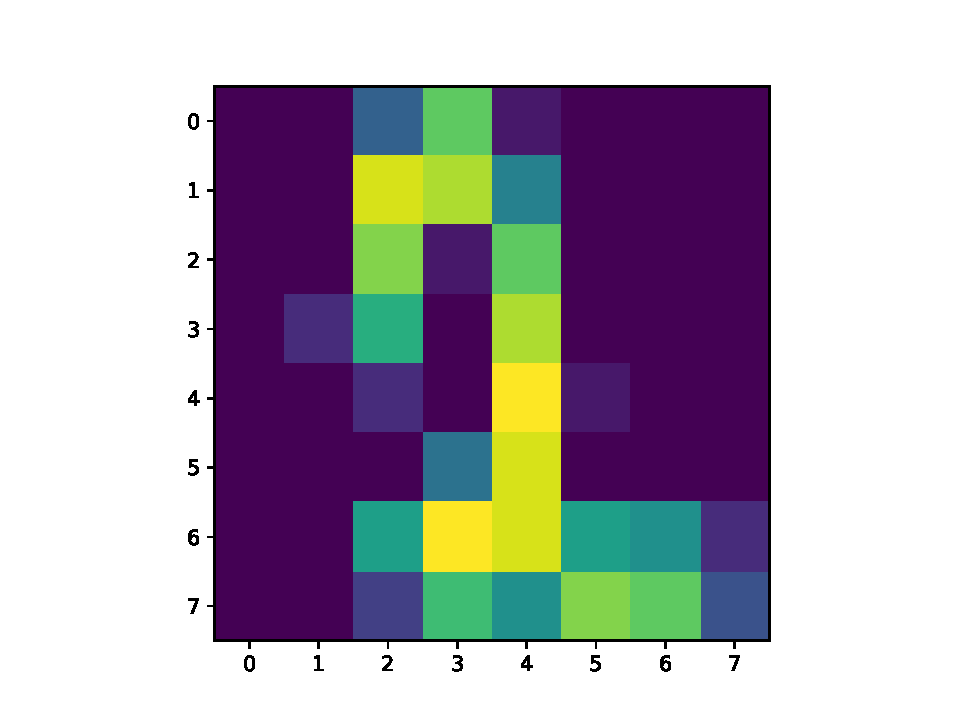
\includegraphics[width=0.5\textwidth]{sample_12}
    	\label{fig:sample_12}
    \end{figure}

    \url{https://scikit-learn.org/stable/modules/generated/sklearn.datasets.load_digits.html} 
\end{frame}

\section{Feature maps}%
\label{sec:Feature maps}

\begin{frame}

    \exercice{}Can we use a linear classifier on this dataset ? What train and test accuracy do we expect ?

\begin{figure}[htpb]
    \centering
    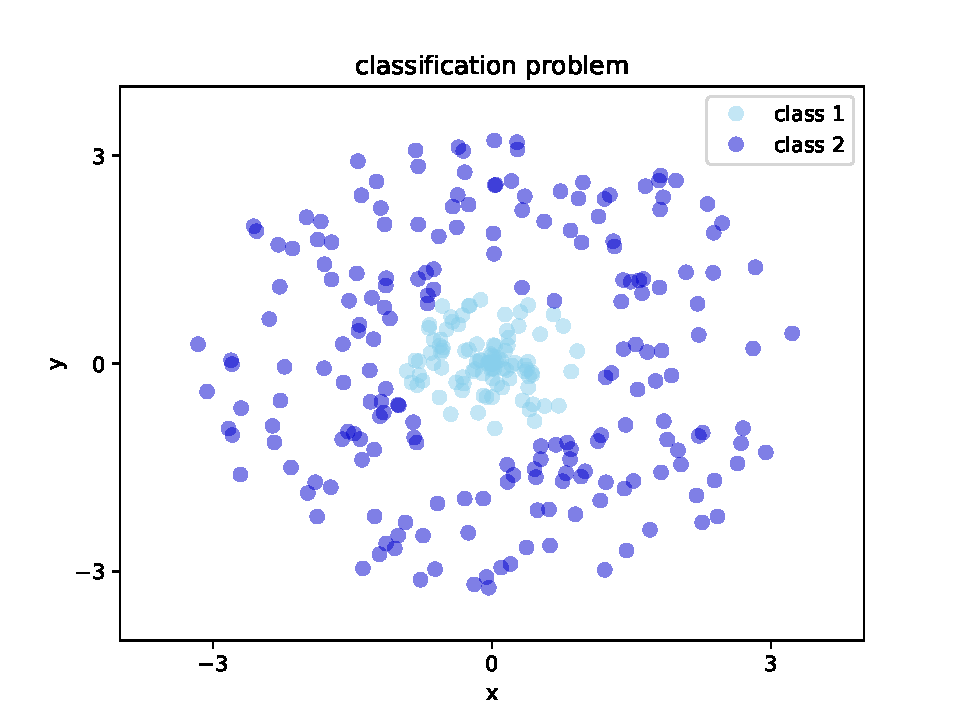
\includegraphics[width=0.8\textwidth]{circle}
    \label{fig:circle}
\end{figure}

\end{frame}

\begin{frame}{Vanilla logistic regression}
\begin{figure}[htpb]
	\centering
	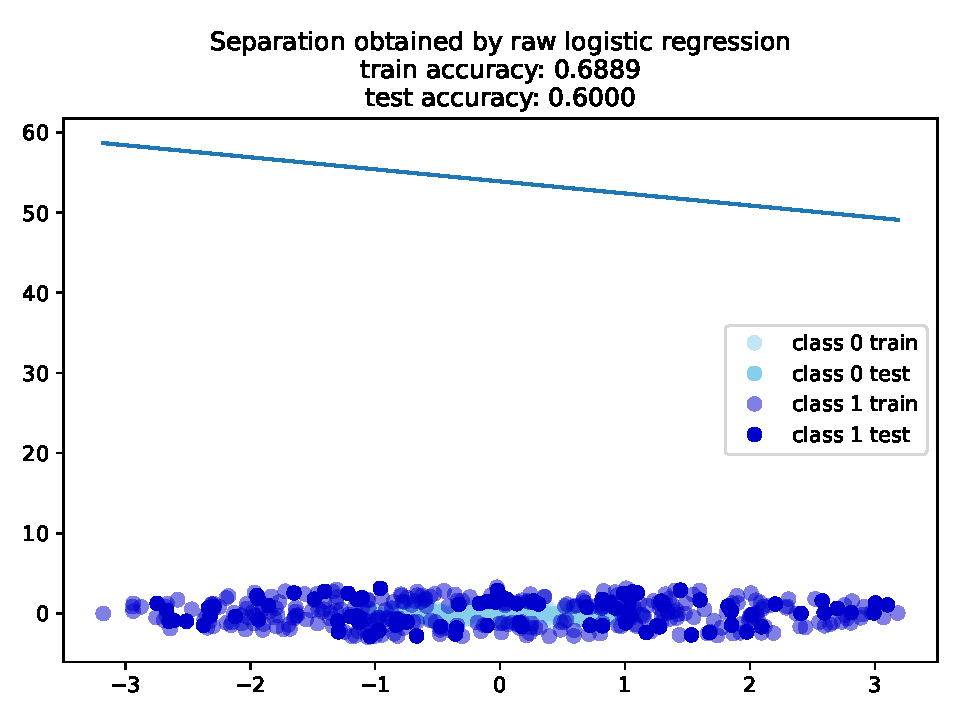
\includegraphics[width=0.5\textwidth]{vanilla_lr}
	\caption{}
	\label{fig:vanilla_lr}
\end{figure}

    File: \textbf{code/day\textunderscore 2/1\textunderscore logistic\textunderscore regression/feature\textunderscore maps/vanilla\textunderscore lr.py}. 
\end{frame}

\begin{frame}{Feature maps}

    \exercice{}Could we \textbf{transform the data} and then apply a logistic regression on them in order to have good train and test accuracies ?

\begin{figure}[htpb]
    \centering
    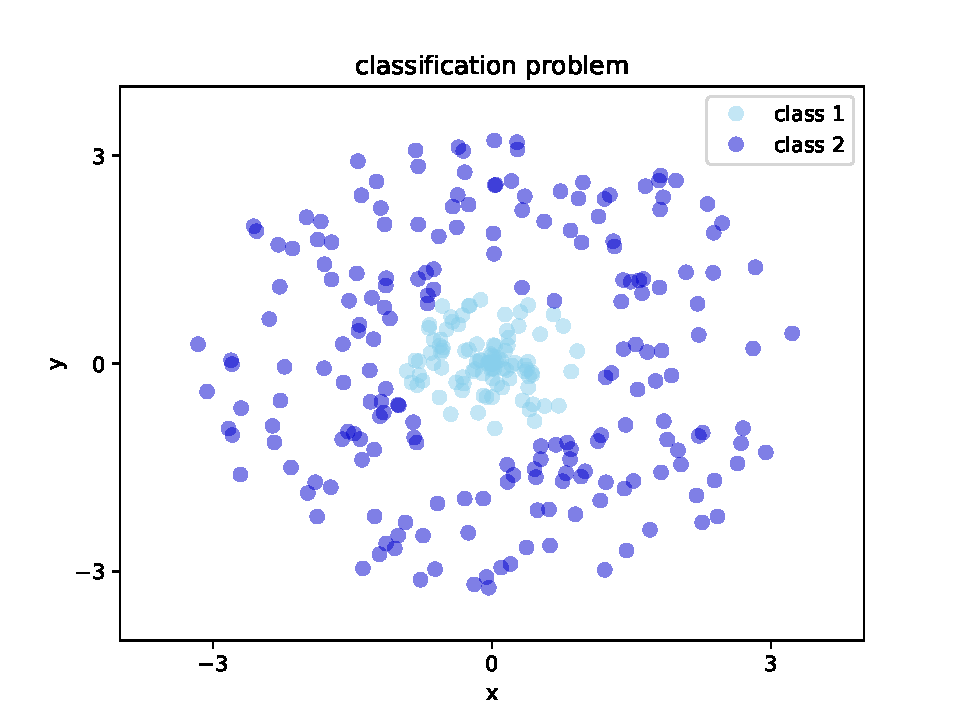
\includegraphics[width=0.5\textwidth]{circle}
    \label{fig:circle}
\end{figure}


Use \textbf{feature\textunderscore maps\textunderscore lr.py} in order to transform the data and correctly classify them with logistic regression.


\end{frame}

\end{document} 
